\documentclass{beamer}
%
% Choose how your presentation looks.
%
% For more themes, color themes and font themes, see:
% http://deic.uab.es/~iblanes/beamer_gallery/index_by_theme.html
%
\mode<presentation>
{
  \usetheme{default}      % or try Darmstadt, Madrid, Warsaw, ...
  \usecolortheme{crane} % or try albatross, beaver, crane, ...
  \usefonttheme{structurebold}  % or try serif, structurebold, ...
  \setbeamertemplate{navigation symbols}{}
  \setbeamertemplate{caption}[numbered]
} 

\usepackage[english]{babel}
\usepackage[utf8x]{inputenc}

\title[ML]{Machine Learning}
\author{Pawel Wocjan}
\institute{University of Central Florida}
\date{Fall 2020}

\begin{document}

\begin{frame}
  \titlepage
\end{frame}

%%%

\begin{frame}{An Iterative Approach}
\begin{itemize}
    \item The figure below depicts the iterative trial-and-error process that machine learning algorithms use to train a model:
\end{itemize}

\bigskip
\includegraphics[width=\textwidth]{images/GradientDescentDiagram.png}
\end{frame}

%%%

\begin{frame}{Gradient Descent}
\begin{itemize}
\item The iterative approach diagram contains a green box ``compute parameter updates.'' 

\medskip    
\item Let us now discuss the gradient descent algorithm that is used to update the parameters.
\end{itemize}
\end{frame}

%%%

\begin{frame}{Gradient Descent}
\begin{itemize}
\item We consider the linear regression model 

$$\hat{y}=f_w(x) = w_1 x_1 + w_2 x_2 + \ldots + w_n x_n + b$$

\medskip
where $w=(w_0, w_1,\ldots,w_n)$.
\end{itemize}
\end{frame}

%%%

\begin{frame}{Gradient Descent}
\begin{itemize}
\item The loss function (mean squared error)

$$\mathcal{L} : \mathbb{R}^{n+1} \rightarrow \mathbb{R}$$ 

\medskip
depends on the parameters $n+1$ parameters $b, w_1, \ldots, w_n$.

\medskip
\item The loss is given by

\begin{align*} 
\mathcal{L} 
&= \frac{1}{m} \sum_{i=1}^m \frac{1}{2} (\hat{y}^{(i)} - y^{(i)})^2 \\
&= \frac{1}{m} \sum_{i=1}^m \frac{1}{2} (f_w(x^{(i)} - y^{(i)})^2 \\
&= \frac{1}{m} \sum_{i=1}^m \frac{1}{2} \left( \sum_{j=1}^n w_j x_j + b- y^{(i)} \right)^2 
\end{align*}

\end{itemize}
\end{frame}

%%%

\begin{frame}{Gradient Decent}
\begin{itemize}
\item For $n=1$, the loss function $\mathcal{L}$ depends on two parameters -- the bias term $b=w_0$ and the weight $w_1$ -- and defines a surface in 3D.

\medskip
\item For $n>1$, the loss function $\mathcal{L}$ cannot be visualized so easily.
\end{itemize}
\end{frame}

%%%

\begin{frame}{Gradient Decent}
\begin{itemize}
\item To simplify the plots, we assume that $n=1$ and the bias term $b=w_0$ is fixed to be $0$.  

\medskip
\item Then, the loss function $\mathcal{L}$ depends only on $w_1$ and defines a curve. 
\end{itemize}
\end{frame}

%%%

\begin{frame}{Gradient Descent}
\begin{itemize}
\item The resulting plot of the loss function $\mathcal{L}$ is be convex. 

\medskip
\item Simply speaking, it means that it is bowl-shaped like this:
\end{itemize}

%\vspace*{-0.5cm}
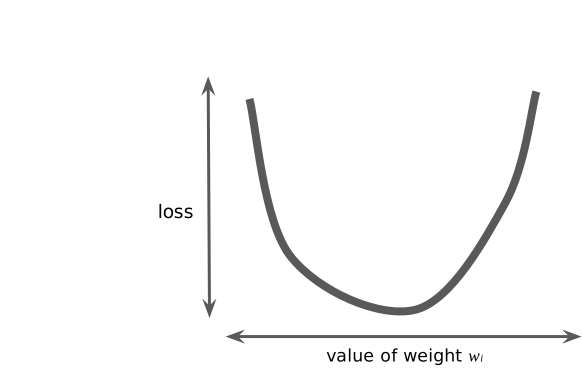
\includegraphics[width=0.9\textwidth]{images/convex.png}
\end{frame}

%%%

\begin{frame}{Gradient Descent}
\begin{itemize}
\item It turns out that even in the general case the loss function $\mathcal{L}$ is convex.

\medskip
\item This is important because problems have only one minimum.

\medskip    
\item Calculating the loss function for all parameter values $w_0,\ldots,w_n\in\mathbb{R}^{n+1}$ would be an inefficient way of finding the minimum.

\medskip    
\item Let's examine a better mechanism -- very popular in machine learning -- called {\bf gradient descent}.
\end{itemize}
\end{frame}

%%%

\begin{frame}{Gradient Descent}
\begin{itemize}
\item The first stage in gradient descent is to pick a starting value. 

\medskip
\item The starting point doesn't matter much; therefore, many algorithms simply set $w_i=0$ or set the $w_i$ to random values.
\end{itemize}

\includegraphics[width=0.9\textwidth]{images/GradientDescentStartingPoint.png}
\end{frame}

%%%

\begin{frame}{Gradient Descent}
\begin{itemize}
\item The gradient descent algorithm then calculates the gradient of the loss function $\mathcal{L}$ at the starting point. 

\medskip
\item The gradient 

$$\nabla\mathcal{L}\in\mathbb{R}^{n+1}$$ 

is a vector whose entries 

$$(\nabla\mathcal{L})_i$$ 

are given by the partial derivatives 

$$\partial \mathcal{L}/\partial w_i$$ 

of the loss function $\mathcal{L}$ with respect to the weights $w_i$.
\end{itemize}
\end{frame}

%%%

\begin{frame}{Gradient Descent}
\begin{itemize}
\medskip    
\item The $\nabla\mathcal{L}$ gradient has both a direction and a magnitude.

\medskip    
\item The gradient points which way is ``warmer'' or ``colder.'' 

\medskip
\item The gradient always points in the direction of steepest increase in the loss function. 

\medskip 
\medskip For the case $n=1$ and the bias $w_0=b$ is fixed to be $0$, the gradient of the loss function $\mathcal{L}$ is simply the slope of the curve $\mathcal{L}$, that is, the derivative with respect to $w_1$.
\end{itemize}
\end{frame}


%%%

\begin{frame}{Gradient Descent}
\begin{itemize}
\item The gradient descent algorithm takes a step in the direction of the negative gradient $-\nabla \mathcal{L}$ to reduce the loss.
\end{itemize}

\vspace{0.1cm}
\includegraphics[width=0.9\textwidth]{images/GradientDescentNegativeGradient.png}
\end{frame}

%%%

\begin{frame}{Gradient Descent}
\begin{itemize}
\item More precisely, the gradient descent algorithm updates the starting point as follows:

\vspace{-0.25cm}

$$ w \leftarrow w - \alpha \nabla\mathcal{L} $$

where $\alpha$ is the learning rate.
\end{itemize}
\includegraphics[width=0.9\textwidth]{images/GradientDescentGradientStep.png}
\end{frame}

%%%

\begin{frame}{Key Terms}
\begin{itemize}
    \item gradient
    \item gradient descent
    \item step
\end{itemize}
\end{frame}


\subsection{Learning Rate}

\begin{frame}{Learning Rate}
\begin{itemize}
\item The gradient vector has both a direction and a magnitude. 

\medskip
\item The gradient descent algorithm multiplies the gradient by a scalar known as the learning rate (also sometimes called step size) to determine the next point. 
\end{itemize}
\end{frame}

%%%

\begin{frame}{Learning Rate}
\begin{itemize}
\item The learning rate is a so-called {\bf hyperparameter}. 

\medskip
\item A hyperparameter is a parameter that is external to the model.
\end{itemize}
\end{frame}

%%%

\begin{frame}{Learning Rate}
\begin{itemize}
\item If the learning rate that is too small, learning will take too long:
\end{itemize}
\includegraphics[width=0.9\textwidth]{images/LearningRateTooSmall.png}
\end{frame}


%%%

\begin{frame}{Learning Rate}
\begin{itemize}
\item If the learning rate is too large, the next point will perpetually bounce haphazardly across the bottom of the well:
\end{itemize}
\includegraphics[width=0.9\textwidth]{images/LearningRateTooLarge.png}
\end{frame}

%%%

\begin{frame}{Learning Rate}
\begin{itemize}
\item There's a Goldilocks learning rate for every linear regression problem.
\end{itemize}
\includegraphics[width=0.9\textwidth]{images/LearningRateJustRight.png}
\end{frame}

%%%

\begin{frame}{Key Terms}
\begin{itemize}
\item hyperparameter
\item learning rate
\item step size
\end{itemize}
\end{frame}

\end{document}